\maketitlesupplementary
This supplementary document complements the main paper by providing extended qualitative and quantitative analyses to further demonstrate the capabilities of our proposed GOGS framework. Specifically, it expands on the experimental results presented in Sec.~\textcolor{red}{5} of the main paper, including comprehensive visualizations of decomposed model outputs across diverse reflective objects, comparative assessments of recovered environment illumination maps, and extensive relighting scenarios under novel illumination conditions. Additionally, we discuss current methodological limitations and future work.
\section{Foundation Models}
To mitigate geometric ambiguities under specular surfaces, we leverage foundation models~\cite{Ke_Obukhov_Huang_Metzger_Daudt_Schindler_2023, garcia2025fine} trained on large-scale datasets for monocular depth and normal estimation. These models generate robust geometric predictions by inferring scene geometry from single-view images through learned priors, bypassing the need for multi-view consistency. As demonstrated in Fig.~\ref{fig:predictions}, the predicted depth and normal maps accurately capture surface details across diverse materials including highly reflective regions. The predictions remain robust to complex specular interference and provide reliable pseudo-ground truth for geometric supervision. This capability stems from foundation models' exposure to massive real-world variations during pretraining, enabling them to disambiguate lighting-surface ambiguities that degrade traditional multi-view reconstruction.

\begin{figure}[b!]
    \centering
    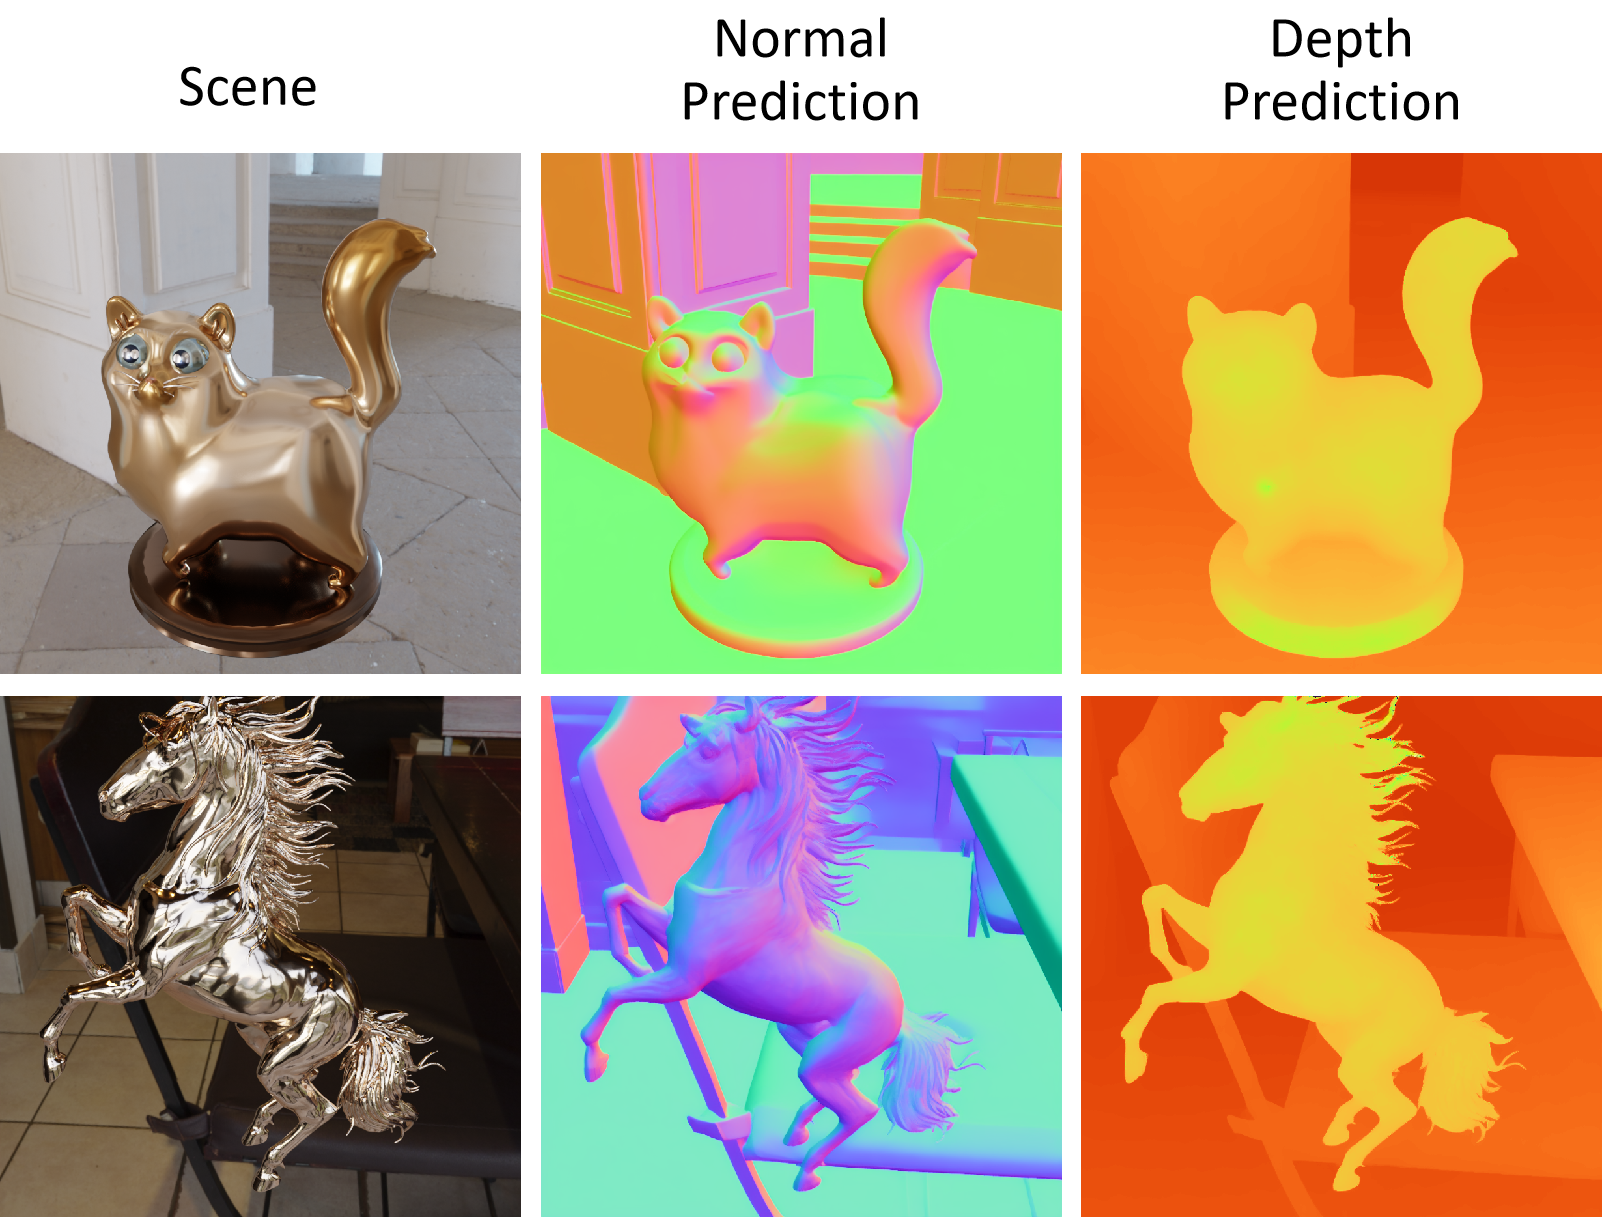
\includegraphics[width=0.9\linewidth]{res/predictions.png}
    \captionsetup{width=0.9\linewidth}
    \caption{Foundation models generate precise depth and normal predictions resilient to specular interference. }
    \label{fig:predictions}
\end{figure}

It is worth noting that two key factors introduce non-determinism. First, depth and normal priors from external foundation models exhibit inherent randomness during inference, leading to minor variations in predicted geometric cues across repeated runs; second, the depth loss (Eq.~\textcolor{red}{9}), which solves for scale $\omega$ and shift $b$ via least squares optimization—is highly sensitive to minimal distributional discrepancies between rendered depth and priors, and such discrepancies can yield non-unique solutions for $\omega$ and $b$, causing fluctuations in alignment parameters during each iteration. These small variations alter the direction of gradient updates, which amplify over time and ultimately result in differences in the final geometric reconstructions.


\begin{figure}[b!]
    \centering
    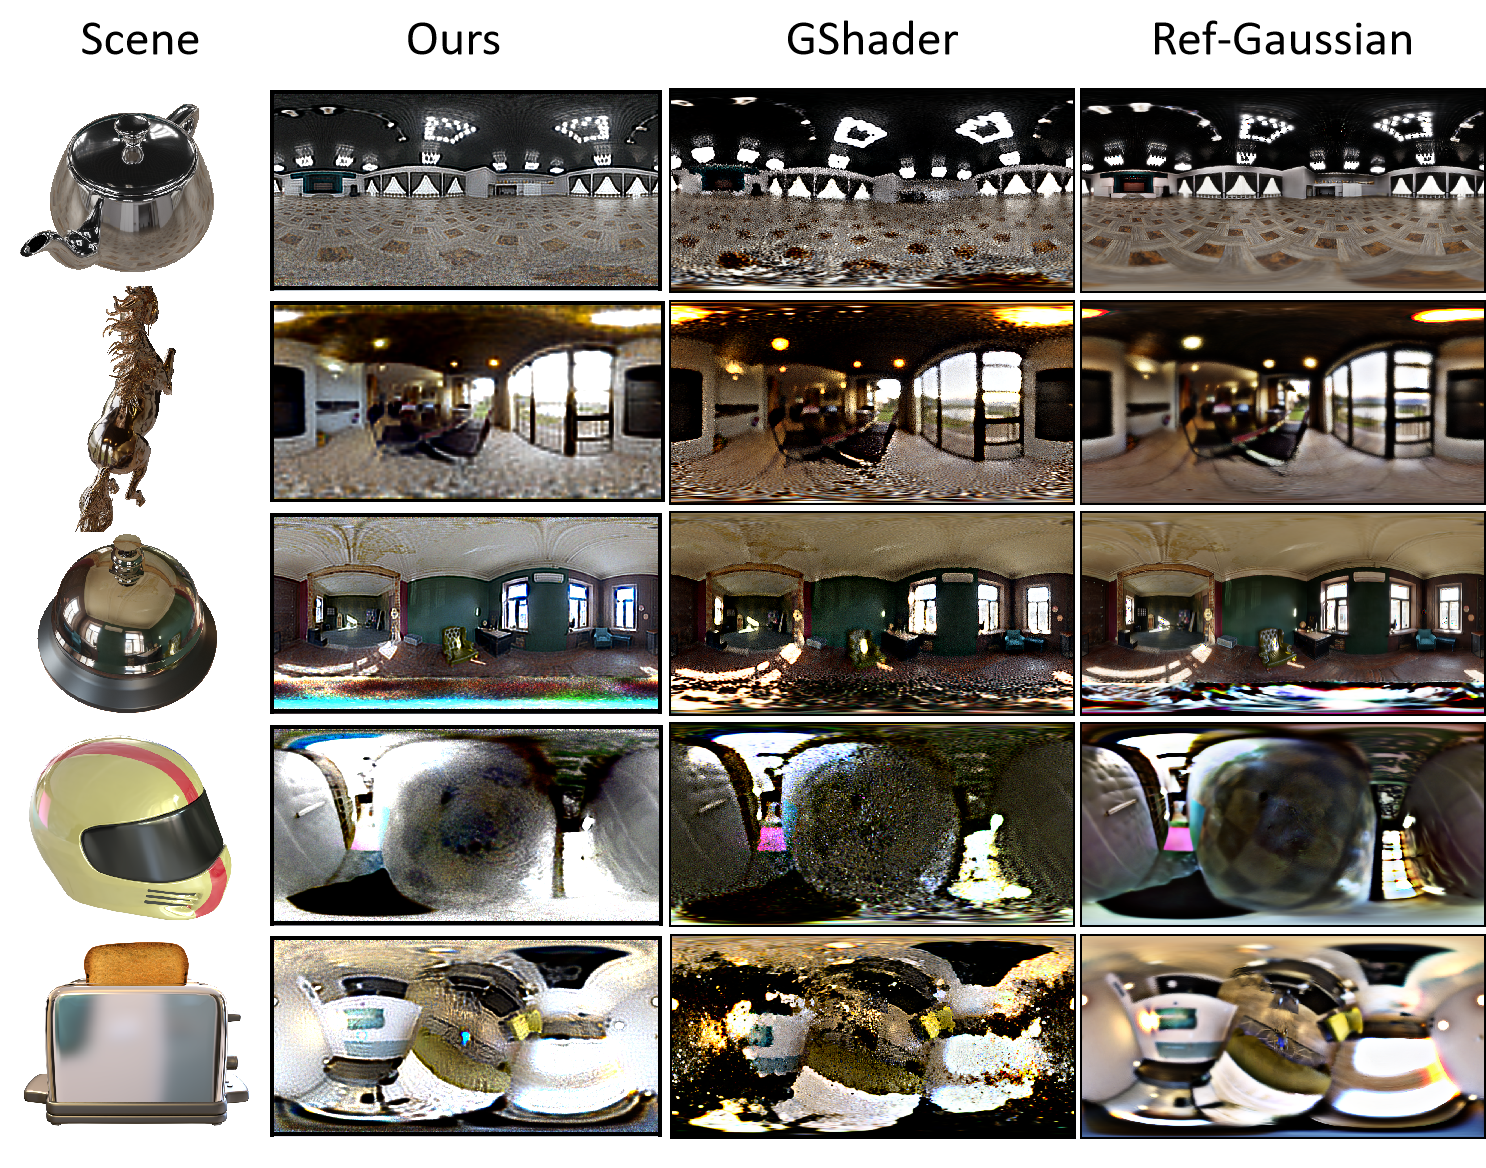
\includegraphics[width=1\linewidth]{res/envmap_compa_more.png}
    \captionsetup{width=0.9\linewidth}
    \caption{Estimated environment maps for reflective object scenes. Our method consistently produces sharper, more artifact-free maps with clearer environmental details compared to competing approaches.}
    \label{fig:envmap_compa_more}
\end{figure}

\begin{figure*}[h!]
    \centering
    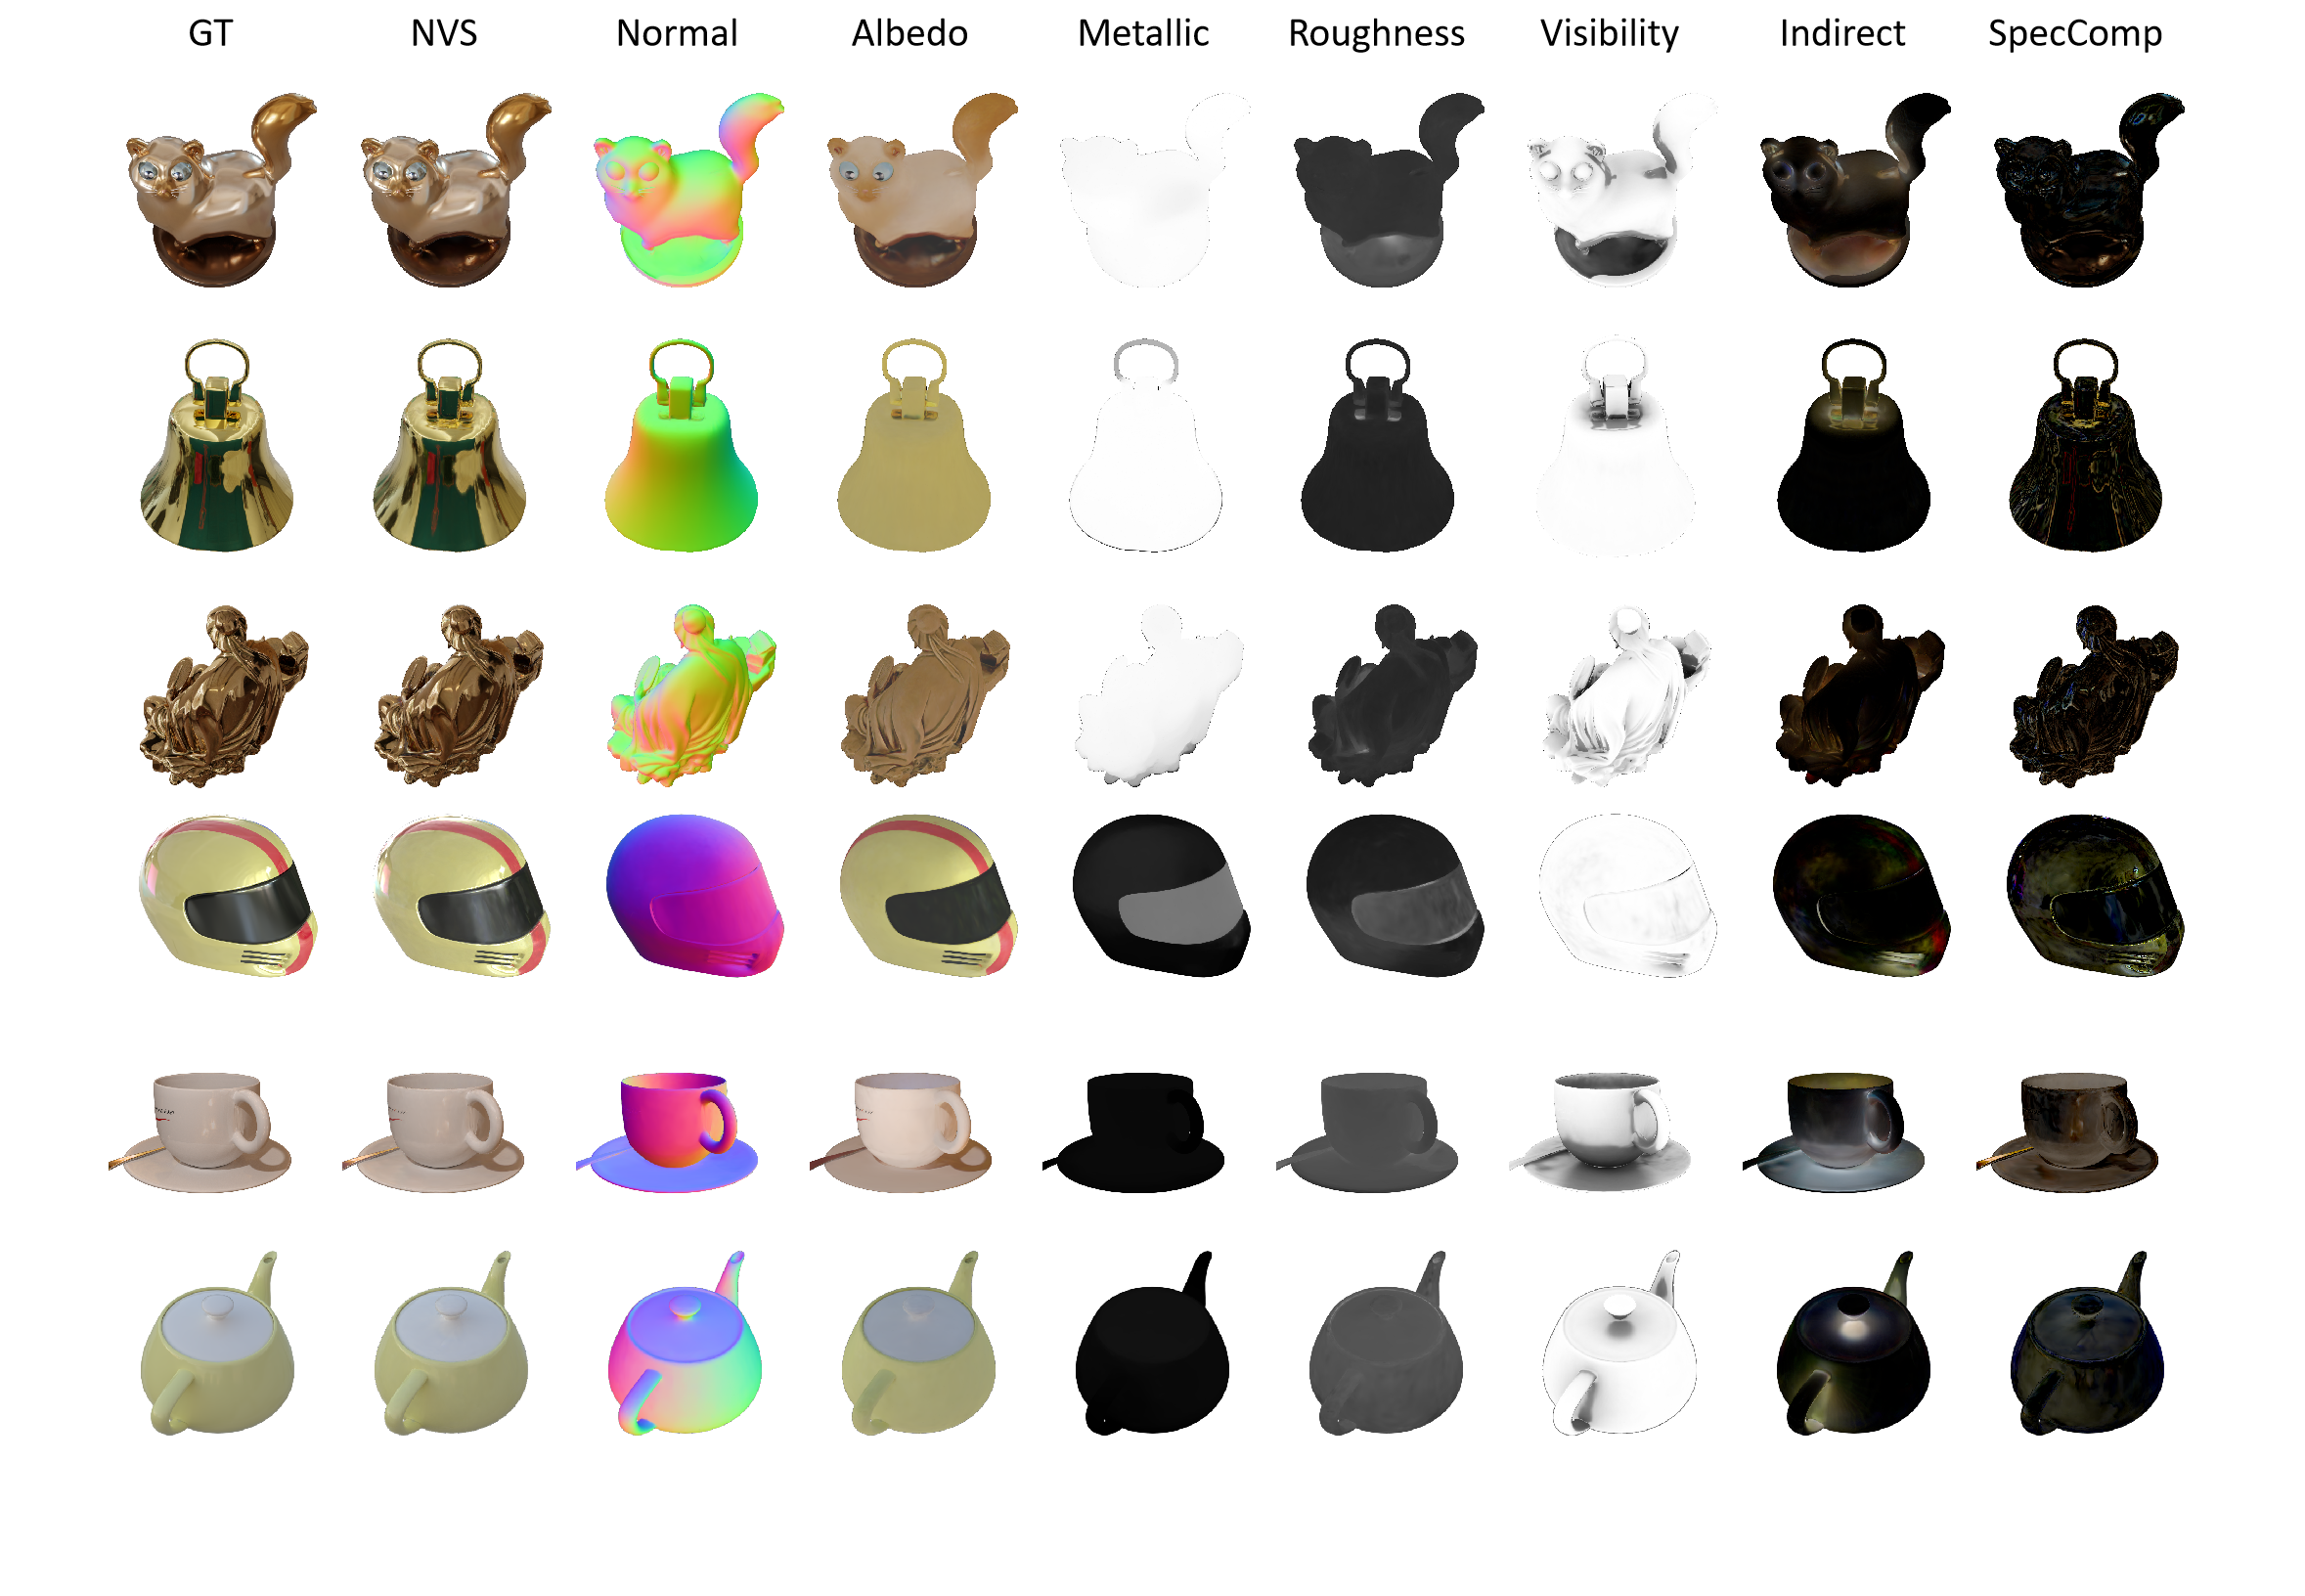
\includegraphics[width=1\linewidth]{res/results_more.png}
    \captionsetup{width=0.9\linewidth}
    \caption{Outputs of our model including ground truth (GT), novel view synthesis (NVS), surface normals (visualized with pseudo-colors), albedo, metallic, roughness, visibility, indirect illumination, and specular compensation (SpecComp).}
    \label{fig:results_more}
\end{figure*}

\section{Comparison}
{
\setlength{\parindent}{0pt} % 只在当前分组内有效
\textbf{Model Outputs.}  
In Fig.~\ref{fig:results_more}, we present detailed output decompositions of our model applied to reflective objects. From left to right, we show the ground truth (GT) for comparison, our model’s novel view synthesis (NVS) results, pseudo-colored surface normals (for enhanced geometric clarity), albedo (diffuse color), metallic, roughness, visibility maps (encoding direct illumination access), indirect illumination, and specular compensation (SpecComp) outputs. These results demonstrate our method’s ability to effectively disentangle geometry (normals), material properties (albedo, metallic, roughness), and illumination (visibility, indirect, specular compensation) during inverse rendering. By separating these components, our model enables high-quality reconstruction, photorealistic novel view synthesis, and high-fidelity relighting—critical for handling reflective surfaces where traditional methods often exhibit limitations. The disentangled illumination and material outputs, in particular, allow precise adjustment of lighting conditions without compromising surface appearance, a key advantage for applications like product visualization and virtual reality.
}

% Please add the following required packages to your document preamble:
% \usepackage{graphicx}
% \usepackage[table,xcdraw]{xcolor}
% Beamer presentation requires \usepackage{colortbl} instead of \usepackage[table,xcdraw]{xcolor}
\begin{table*}[h!]
\centering
\captionsetup{width=0.9\textwidth}
\caption{Quantitative relighting comparisons on three environment maps (corridor, golf, neon) from Glossy Synthetic~\cite{liu2023nero} using three metrics (PSNR ↑, SSIM ↑~\cite{ssim}, LPIPS ↓~\cite{lpips}), with best results per metric highlighted in red.}
\label{tab:relight_compa}
\resizebox{0.95\textwidth}{!}{%
\begin{tabular}{l|cccc|cccc|cccc}
\hline
\hline
 & \textbf{corridor} & \textbf{golf} & \textbf{neon} & \textbf{avg.} & \textbf{corridor} & \textbf{golf} & \textbf{neon} & \textbf{avg.} & \textbf{corridor} & \textbf{golf} & \textbf{neon} & \textbf{avg.} \\ \hline
 & \multicolumn{4}{c|}{PSNR ↑} & \multicolumn{4}{c|}{SSIM↑} & \multicolumn{4}{c}{LPIPS↓} \\ \hline
GShader\cite{jiang2024gaussianshader} & 19.81 & 18.14 & 19.24 & 19.06 & 0.862 & 0.876 & 0.860 & 0.866 & 0.101 & 0.102 & 0.104 & 0.103 \\
Ref-GS\cite{yao2024refgaussian} & 21.83 & 21.69 & 21.36 & 21.63 & 0.900 & \cellcolor[HTML]{FD6864}0.920 & 0.894 & 0.905 & 0.075 & \cellcolor[HTML]{FD6864}0.077 & \cellcolor[HTML]{FD6864}0.082 & \cellcolor[HTML]{FD6864}0.078 \\
IRGS\cite{gu2025irgs} & 22.01 & 21.04 & 20.12 & 21.06 & 0.874 & 0.840 & 0.832 & 0.849 & 0.131 & 0.164 & 0.151 & 0.149 \\
Ours & \cellcolor[HTML]{FD6864}25.75 & \cellcolor[HTML]{FD6864}26.01 & \cellcolor[HTML]{FD6864}22.88 & \cellcolor[HTML]{FD6864}24.89 & \cellcolor[HTML]{FD6864}0.925 & 0.914 & \cellcolor[HTML]{FD6864}0.909 & \cellcolor[HTML]{FD6864}0.916 & \cellcolor[HTML]{FD6864}0.070 & 0.092 & 0.084 & 0.082 \\ \hline
\hline
\end{tabular}%
}
\end{table*}

{
\setlength{\parindent}{0pt} % 只在当前分组内有效
\textbf{Environment Maps.}  
In Fig.~\ref{fig:envmap_compa_more}, we present a comparison of estimated environment maps for various reflective object scenes (left column), including a teapot, horse, car, and helmet. From left to right after the scene column, we show results from our model, GShader~\cite{jiang2024gaussianshader}, Ref-Gaussian(Ref-GS)~\cite{yao2024refgaussian}. Our method effectively disentangles illumination from scene geometry and material properties, resulting in sharper environment maps with fewer artifacts—such as the crisp ceiling patterns in the teapot scene, distinct window frames in the horse scene—compared to GShader’s slightly blurred outputs~\cite{jiang2024gaussianshader} and Ref-Gaussian’s muted details~\cite{yao2024refgaussian}. Notably, these methods exhibit severe noise and color distortion in most cases (e.g., the car and helmet scenes), while our model maintains consistent clarity across all scenes. These results demonstrate our method’s superior ability to recover high-fidelity environment illumination, which is critical for realistic rendering and relighting of reflective surfaces—an essential capability for applications like product visualization and virtual reality.
}


\begin{figure}[]
    \centering
    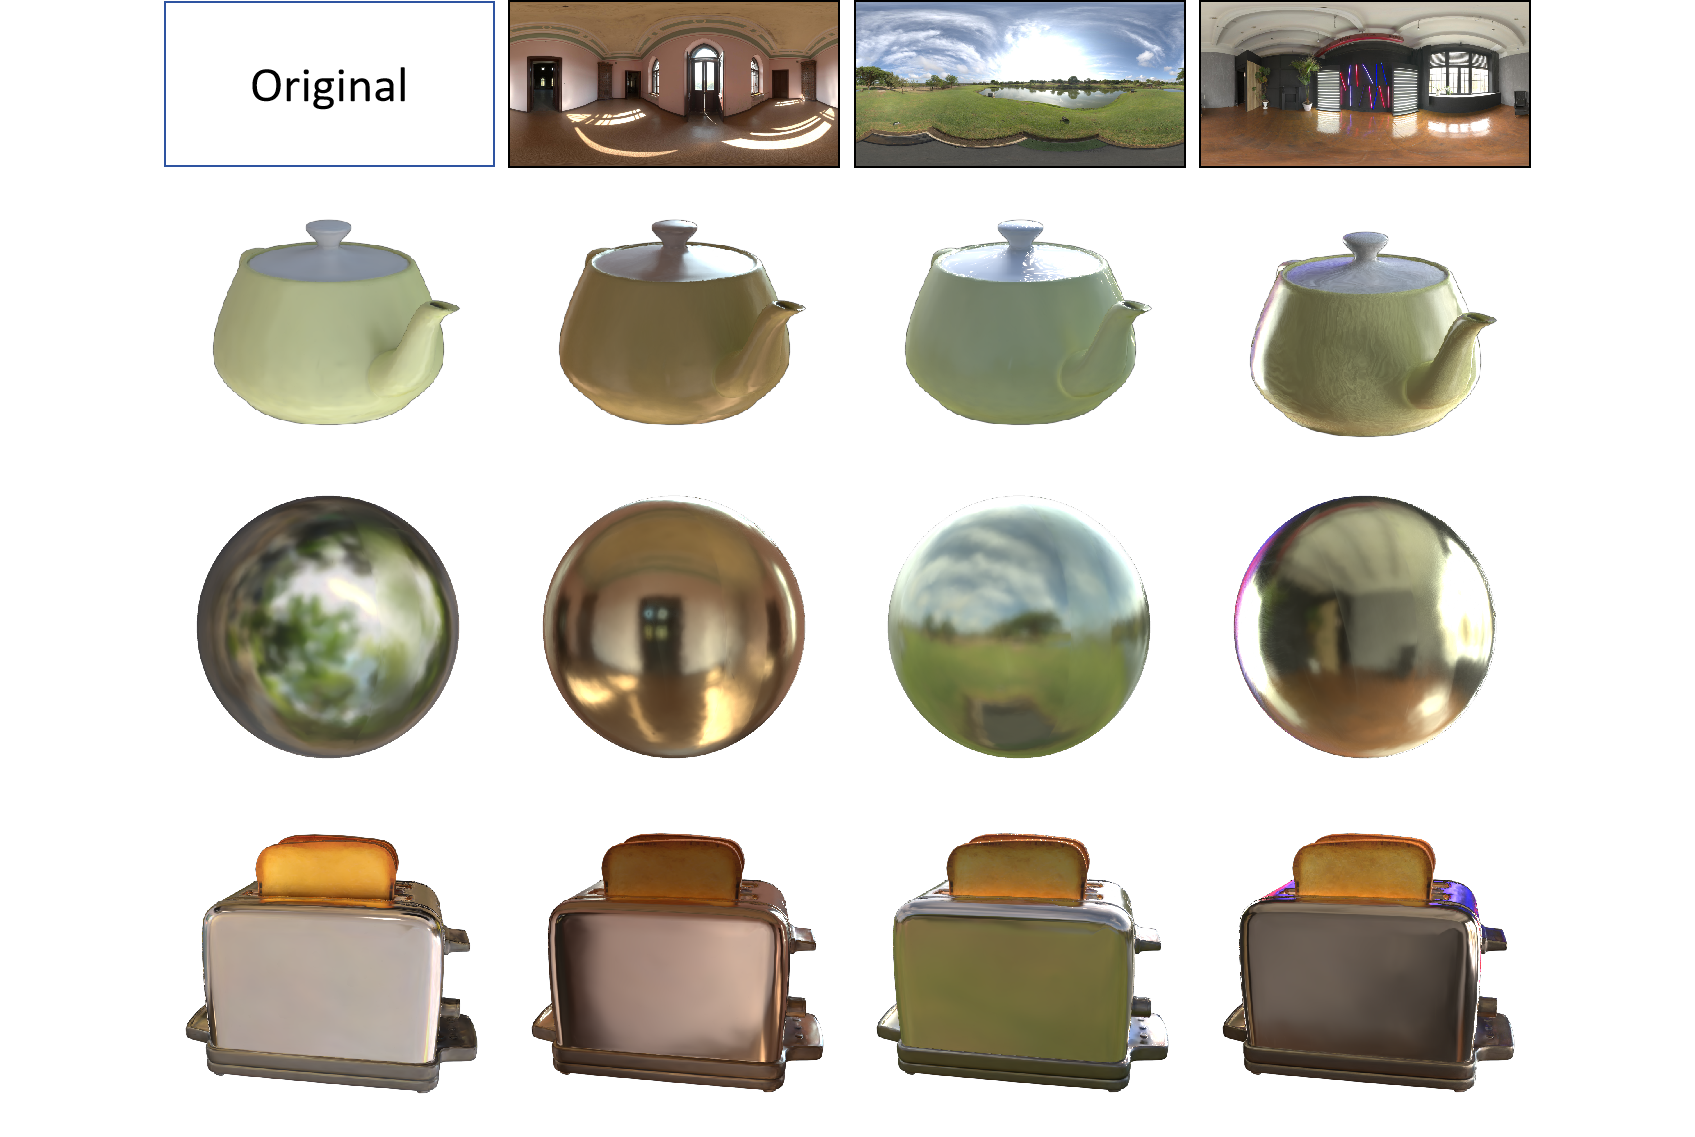
\includegraphics[width=1\linewidth]{res/relight_results_more.png}
    \captionsetup{width=0.9\linewidth}
    \caption{Our GOGS framework generates high-fidelity relighting results across diverse objects, consistently preserving geometric fidelity and material properties while producing sharp, physically plausible specular reflections under novel illumination conditions.}
    \label{fig:relight_results_more}
\end{figure}


{
\setlength{\parindent}{0pt} % 只在当前分组内有效
\textbf{Relighting.}  
In Fig.~\ref{fig:relight_results_more}, we demonstrate GOGS's relighting capabilities across surfaces with diverse reflectance properties. For each exemplar object, we preserve the original rendering under default illumination (leftmost column), followed by relighting under three novel illumination conditions (subsequent columns). Our method consistently disentangles illumination from intrinsic scene properties, maintaining geometric fidelity (e.g., fine structural details) and material characteristics across lighting variations. Relighted outputs exhibit physically accurate reflections: highly specular surfaces precisely mirror environmental features, while matte surfaces retain color/texture consistency.These results validate our model's capability for high-fidelity relighting of arbitrary materials under varied illuminations.
}

Tab.~\ref{tab:relight_compa} summarizes the relighting performance of four methods (GShader~\cite{jiang2024gaussianshader}, Ref-GS~\cite{yao2024refgaussian}, IRGS~\cite{gu2025irgs}, and ours) on three representative environment maps (corridor, golf, neon) using three widely adopted metrics: PSNR↑, SSIM↑~\cite{ssim}, and LPIPS↓~\cite{lpips}. For each metric, we report results on individual environment maps and their average (avg.), with the best results highlighted in red.  
Consistently, our method achieves the highest average PSNR and SSIM across all environment maps, outperforming the second-best method by significant margins. These results validate the effectiveness of our method in disentangling illumination from scene geometry and material properties, which is critical for high-fidelity relighting applications like product visualization and virtual reality.
These results validate our model's capability for high-fidelity relighting of arbitrary materials under varied illuminations.


\section{Limitation}
Our framework has certain limitations requiring further investigation. While optimized for specular reflections, our Monte Carlo importance sampling exhibits suboptimal performance on complex mixed-material surfaces due to differing BRDF characteristics. To address this, future work will focus on adaptive importance sampling techniques capable of handling complex mixed materials and generalizing across material roughness. Additionally, computational costs from our ray tracing implementation and spherical encoding currently preclude real-time applications, despite offering significant speed improvements over NeRF-based methods. Tab.~\ref{tab:time} quantifies this trade-off: our model achieves a training time of 1.33 hours without specular compensation—far faster than NeRF-based ENVIDR (5.84 hours)—but slower than lightweight models like 3DGS-DR (0.35 hours) and GShader (0.48 hours). This aligns with our observation that while we outperform NeRF-based methods, real-time capability remains a challenge. To address this, we plan to accelerate rendering by baking incident radiance through precomputed radiance transfer schemes while maintaining physical accuracy.Finally, while our 2D Gaussian ray tracing approximates visibility and indirect illumination, it remains insufficient for capturing high-fidelity multi-bounce specular inter-reflections. Real-world light transport in glossy surfaces involves theoretically infinite path bounces—a phenomenon prohibitively expensive to simulate using path-tracing in inverse rendering due to its computational burden. To address this limitation, we will explore novel neural network-based approximation techniques for modeling complex light paths.

% Please add the following required packages to your document preamble:
% \usepackage{multirow}
% \usepackage{graphicx}
% \usepackage[table,xcdraw]{xcolor}
% Beamer presentation requires \usepackage{colortbl} instead of \usepackage[table,xcdraw]{xcolor}
\begin{table}[]
\centering
\caption{Quantitative comparison of training time efficiency on the Shiny Blender dataset~\cite{verbin2022refnerf}.}
\label{tab:time}
\resizebox{\columnwidth}{!}{%
\begin{tabular}{c|ccccc}
\hline
\hline
\Large
 & \multicolumn{5}{c}{Model} \\ \cline{2-6} 
\multirow{-2}{*}{\begin{tabular}[c]{@{}c@{}}Efficiency \\ evaluation\end{tabular}} & ENVIDR\cite{liang2023envidr} & 3DGS-DR\cite{ye20243dgsdr} & Ref-GS\cite{yao2024refgaussian} & IRGS\cite{gu2025irgs} & Ours \\ \hline
\begin{tabular}[c]{@{}c@{}}Training \\ time (h)↓\end{tabular} & 5.84 & \cellcolor[HTML]{FD6864}0.35 & 0.58 & 0.70 & 1.33 \\ \hline
\hline
\end{tabular}%
}
\end{table}

